Deep learning represents a new programming paradigm: instead of deterministic
programs, users design models and ``simply'' train them with data. In this
metaphor, deep learning is a meta-programming form, where \emph{coding} is
replaced by \emph{training}. Here, we ponder the question how we can provide
more insight into this process by building a \emph{debugger} specifically
designed for deep learning.

Debuggers are crucial for traditional software development. When things fail,
they provide access to the internal workings of the code, allowing a look ``into
the box''. This is much more efficient than re-running the program with
different inputs. And yet, deep learning is arguably closer to the latter. If
the attempt to train a deep net fails, a machine learning engineer faces various
options: should they change the training hyperparameters (how?); the optimizer
(to which one?); the model (how?); or just re-run with a different seed? Machine
learning toolboxes provide scant help to guide these decisions.

Of course, traditional debuggers can be applied to deep learning. They will give
access to every single weight of a neural net, or the individual pixels of its
training data. But this rarely yields insights towards successful training.
Extracting meaningful information requires a statistical approach and
distillation of the bewildering complexity into a manageable summary. Tools like
\tensorboard \citep{abadi2016tensorflow} or \wandb \citep{biewald2020experiment} were built in part
to streamline this visualization. Yet, the quantities that are widely monitored
(mainly train/test loss \& accuracy), provide only scant explanation for
relative differences between multiple training runs, because \emph{they do not
  show the network's internal state}. \Cref{cockpit::fig:LINE} illustrates how such
established learning curves can describe the \emph{current} state of the model
-- whether it is performing well or not -- while failing to inform about
training state and dynamics. They tell the user \emph{that} things are going
well or badly, but not \emph{why}. The situation is similar to flying a plane by
sight, without instruments to provide feedback. It is not surprising, then, that
achieving state-of-the-art performance in deep learning requires expert
intuition, or plain trial \& error.

\begin{figure*}[!t]
  \centering
  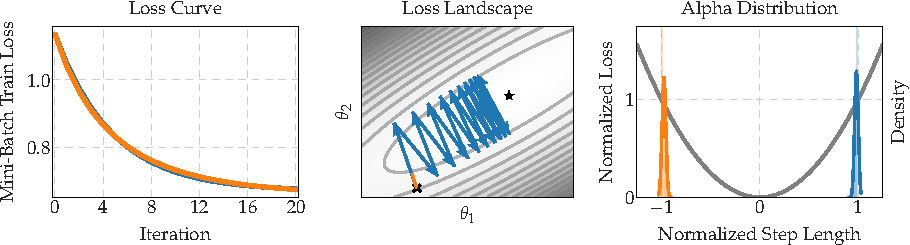
\includegraphics{../repos/cockpit-paper/fig/02_LINE/output/LINE_thesis-wide}
  \caption{\textbf{Illustrative example: learning curves do not tell the whole
      story}. Two different optimization runs
    (\textcolor{sns_orange}{\textbf{---}}/\textcolor{sns_blue}{\textbf{---}})
    can lead to virtually the same loss curve (\textit{left}). However, the
    actual optimization trajectories (\textit{middle}), exhibit vastly different
    behaviors. In practice, the trajectories are intractably large and cannot be
    visualized directly. Recommendable actions for both scenarios
    (\textcolor{sns_orange}{increase}/\textcolor{sns_blue}{decrease} the
    learning rate) cannot be inferred from the loss curve. The
    $\alpha$-distribution, one \cockpit instrument (\textit{right}), not only
    clearly distinguishes the two scenarios, but also allows for taking
    decisions how the learning rate should be adapted. See
    \Cref{cockpit::sec:alpha_exp} for further details.}\label{cockpit::fig:LINE}
\end{figure*}

\begin{figure*}[!t]
  \centering
  % trim={<left> <lower> <right> <upper>}, clip
  \Cshadowbox{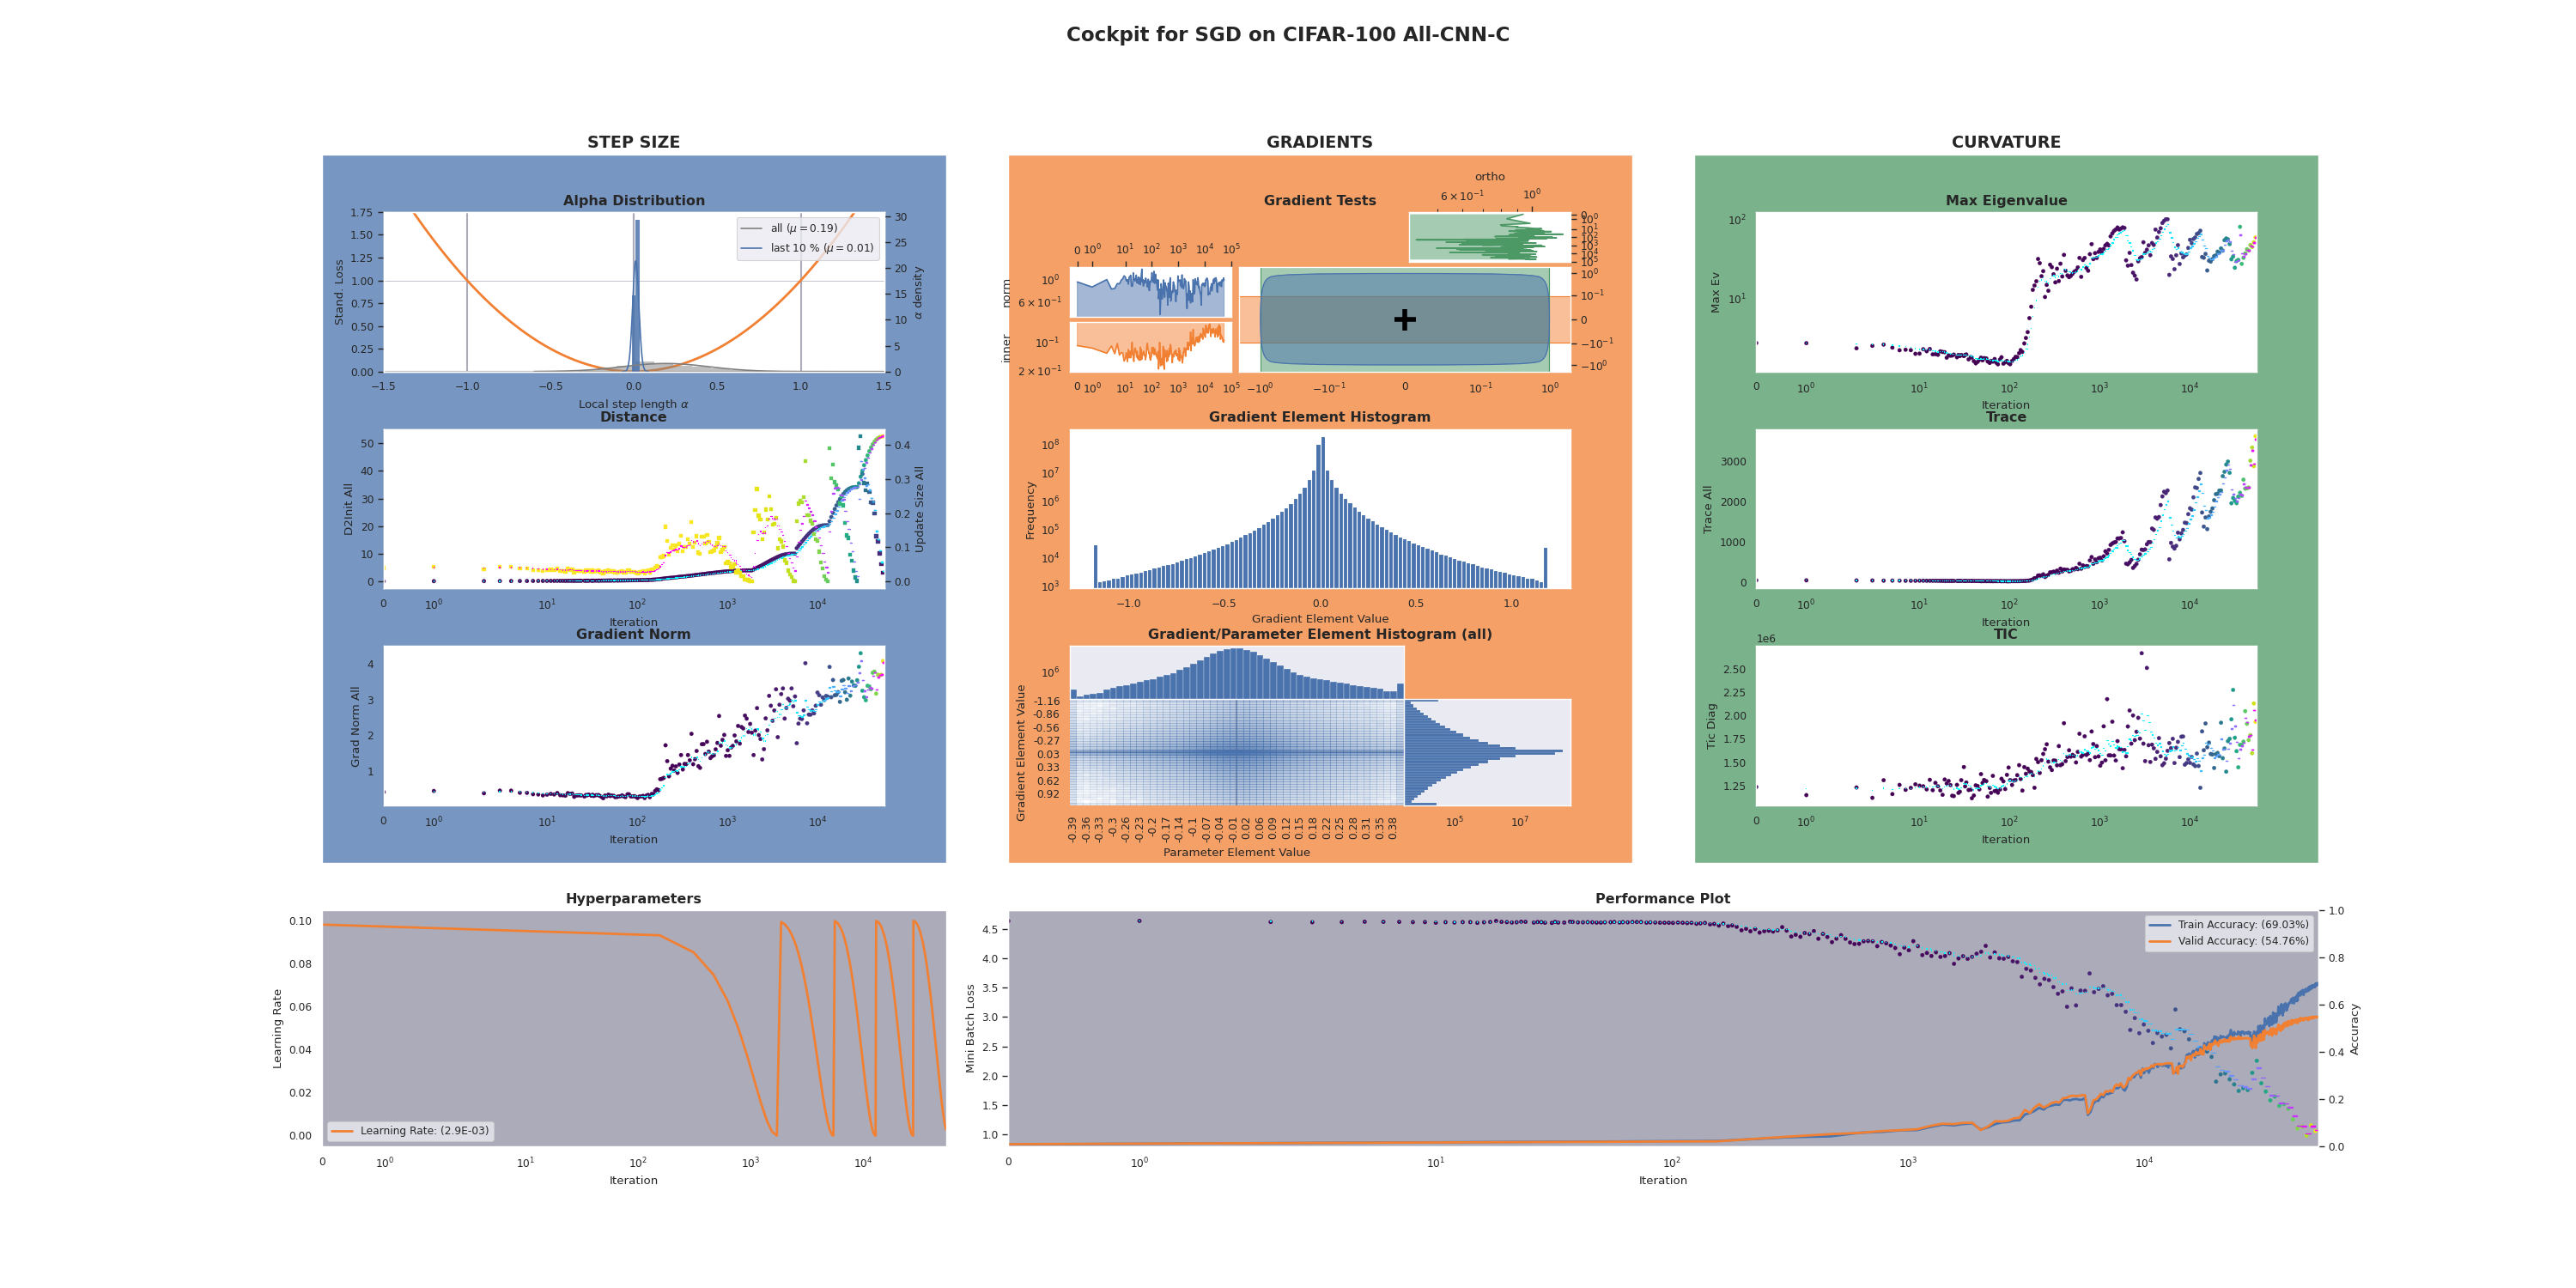
\includegraphics[width=0.97\linewidth, trim={7cm 2.5cm 5cm
      0.5cm}, clip]{../repos/cockpit-paper/tex/fig/10_showcase/cifar100_allcnnc_log.png}}
  \vspace{0.5ex}
  \caption{\textbf{Screenshot of \cockpittitle's full view} while training the
    \allcnnc \citep{springenberg2015striving} on \cifarhun with \sgd using a cyclical
    learning rate schedule. This figure and its labels are not meant to be
    legible, but rather give an impression of \cockpit's user experience. Gray
    panels (bottom row) show the information currently tracked by most
    practitioners. The individual instruments are discussed in
    \Cref{cockpit::sec:instruments}, and observations are described in
    \Cref{cockpit::sec:showcase}. An animated version can be found in the accompanying
    Github repository.}
  \label{cockpit::fig:showcase}
\end{figure*}

We aim to enrich the deep learning pipeline with a visual and statistical
debugging tool that uses newly proposed observables as well as several
established ones (\Cref{cockpit::sec:instruments}). We leverage and augment recent
extensions to AD (\ie \backpack \citep{dangel2020backpack} for
\pytorch \citep{paszke2019pytorch}) to efficiently access second-order statistical (\eg
gradient variances) and geometric (\eg Hessian) information. We show how these
quantities can aid the deep learning engineer in tasks, like learning rate
selection, as well as detecting common bugs with data processing or model
architectures (\Cref{cockpit::sec:experiments}).

Concretely, we introduce \cockpit, a flexible and efficient framework for
online-monitoring these observables during training in carefully designed plots
we call ``instruments'' (\Cref{cockpit::fig:showcase}). To practical, such
visualization must have a manageable computational overhead. We show that
\cockpit scales well to real-world deep learning problems (see
\Cref{cockpit::fig:showcase} and \Cref{cockpit::sec:showcase}). We also provide
three different configurations of varying computational complexity and
demonstrate that their instruments keep the computational cost \textit{well
  below} a factor of $2$ in run time (\Cref{cockpit::sec:benchmark}). It is
available as open-source code, extendable, and seamlessly integrates into
existing \pytorch training loops (\Cref{cockpit::app:code_example}).

%%% Local Variables:
%%% mode: latex
%%% TeX-master: "../thesis"
%%% End:
